\documentclass[conference]{IEEEtran}
\IEEEoverridecommandlockouts
\usepackage{cite}
\usepackage{amsmath,amssymb,amsfonts}
\usepackage{algorithmic}
\usepackage{graphicx}
\usepackage{textcomp}
\usepackage{xcolor}
\usepackage[T1]{fontenc}
\usepackage[utf8]{inputenc}
\usepackage[brazil]{babel}
\usepackage{booktabs}
\usepackage{url}
\def\BibTeX{{\rm B\kern-.05em{\sc i\kern-.025em b}\kern-.08em T\kern-.1667em\lower.7ex\hbox{E}\kern-.125emX}}

\makeatletter
\newcommand{\linebreakand}{%
  \end{@IEEEauthorhalign}
  \hfill\mbox{}\par
  \mbox{}\hfill\begin{@IEEEauthorhalign}
}
\makeatother

\begin{document}

\title{Um Sistema de Segmenta\c{c}\~ao de Clientes de Shopping baseado em K-Means com Sele\c{c}\~ao Criteriosa de Grupos e Gera\c{c}\~ao de Personas Acion\'aveis}

\author{
\IEEEauthorblockN{Chistian Daniel Pereira da Silva}
\IEEEauthorblockA{\textit{Bacharelado em Tecnologia da Informação} \\
\textit{Instituto Metrópole Digital (IMD), UFRN}\\
Natal/RN, Brasil}
\and
\IEEEauthorblockN{Enock Gomes Neto}
\IEEEauthorblockA{\textit{Bacharelado em Tecnologia da Informação} \\
\textit{Instituto Metrópole Digital (IMD), UFRN}\\
Natal/RN, Brasil}

\linebreakand 

\IEEEauthorblockN{Esdras Felipe Chaves Pinto Nascimento e Silva}
\IEEEauthorblockA{\textit{Bacharelado em Tecnologia da Informação} \\
\textit{Instituto Metrópole Digital (IMD), UFRN}\\
Natal/RN, Brasil}
\and
\IEEEauthorblockN{Gabriel Santos da Silveira}
\IEEEauthorblockA{\textit{Bacharelado em Tecnologia da Informação} \\
\textit{Instituto Metrópole Digital (IMD), UFRN}\\
Natal/RN, Brasil}

\linebreakand 

\IEEEauthorblockN{Glauco Ezequiel de Sousa Gonçalves}
\IEEEauthorblockA{\textit{Bacharelado em Tecnologia da Informação} \\
\textit{Instituto Metrópole Digital (IMD), UFRN}\\
Natal/RN, Brasil}
\and
\IEEEauthorblockN{Vitor Fraifer Palhano dos Anjos}
\IEEEauthorblockA{\textit{Bacharelado em Tecnologia da Informação} \\
\textit{Instituto Metrópole Digital (IMD), UFRN}\\
Natal/RN, Brasil}
}

\maketitle

\begin{abstract}
A segmenta\c{c}\~ao de clientes \'e uma tarefa central no varejo, pois permite direcionar a\c{c}\~oes de marketing a grupos com comportamentos de consumo distintos. Este trabalho apresenta um \textit{sistema} completo de segmenta\c{c}\~ao --- e n\~ao apenas a valida\c{c}\~ao de um conjunto de dados --- estruturado como um \textit{pipeline} que recebe atributos demogr\'aficos e comportamentais de clientes e produz personas acion\'aveis. O n\'ucleo do sistema \'e o algoritmo K-Means. Duas contribui\c{c}\~oes t\'ecnicas s\~ao destacadas: (i) a escolha do n\'umero de grupos $k$ combinando tr\^es crit\'erios independentes --- m\'etodo do cotovelo, coeficiente de silhueta e \'indice Calinski-Harabasz --- de modo que a concord\^ancia gere confian\c{c}a e a diverg\^encia se torne objeto de discuss\~ao; e (ii) a tradu\c{c}\~ao de cada grupo em uma persona com recomenda\c{c}\~ao de marketing. Aplicado ao \textit{Mall Customer Segmentation Dataset} (200 clientes), o sistema identificou cinco perfis interpret\'aveis, com coeficiente de silhueta de $0{,}42$, e gerou recomenda\c{c}\~oes de neg\'ocio coerentes com a literatura.
\end{abstract}

\begin{IEEEkeywords}
aprendizado n\~ao-supervisionado, K-Means, segmenta\c{c}\~ao de clientes, silhueta, PCA, personas.
\end{IEEEkeywords}

\section{Introdu\c{c}\~ao}
A capacidade de compreender o comportamento de compra dos consumidores tornou-se um diferencial competitivo para o varejo. Em vez de tratar a base de clientes como um todo homog\^eneo, as empresas buscam dividi-la em grupos com caracter\'isticas semelhantes, pr\'atica conhecida como \textit{segmenta\c{c}\~ao de clientes}. Cada segmento pode ent\~ao receber estrat\'egias de marketing espec\'ificas, o que aumenta a efetividade das campanhas e a satisfa\c{c}\~ao do cliente.

Como na pr\'atica n\~ao se conhecem previamente os r\'otulos dos segmentos, o problema \'e naturalmente abordado por t\'ecnicas de \textit{aprendizado de m\'aquina n\~ao-supervisionado}, em particular por algoritmos de agrupamento (\textit{clustering}). O K-Means~\cite{macqueen1967} \'e o m\'etodo mais empregado nesse contexto por sua simplicidade, efici\^encia e interpretabilidade.

Entretanto, dois desafios pr\'aticos costumam ser subestimados. O primeiro \'e a defini\c{c}\~ao do n\'umero de grupos $k$, par\^ametro que o K-Means n\~ao infere automaticamente e que afeta diretamente a qualidade da solu\c{c}\~ao. O segundo \'e a transforma\c{c}\~ao dos grupos obtidos em informa\c{c}\~ao \'util para o neg\'ocio: um r\'otulo num\'erico de \textit{cluster}, isoladamente, n\~ao orienta a\c{c}\~oes.

Este trabalho aborda ambos os desafios propondo um \textit{sistema} de segmenta\c{c}\~ao com \textit{pipeline} bem definido. As contribui\c{c}\~oes s\~ao: (i) a sele\c{c}\~ao criteriosa de $k$ por meio da combina\c{c}\~ao de tr\^es crit\'erios complementares; e (ii) a gera\c{c}\~ao autom\'atica de personas com recomenda\c{c}\~oes de marketing a partir dos centroides. O sistema foi avaliado sobre o \textit{Mall Customer Segmentation Dataset}.

\section{Trabalhos Relacionados}
O K-Means foi formalizado por MacQueen~\cite{macqueen1967} e permanece, d\'ecadas depois, um dos algoritmos de agrupamento mais utilizados, sobretudo em aplica\c{c}\~oes de marketing e an\'alise de clientes. Para a escolha de $k$, a literatura oferece crit\'erios distintos: o m\'etodo do cotovelo analisa a redu\c{c}\~ao da in\'ercia (soma das dist\^ancias intra-grupo); o coeficiente de silhueta~\cite{rousseeuw1987} mede o qu\~ao bem cada ponto se ajusta ao seu grupo em rela\c{c}\~ao ao grupo vizinho mais pr\'oximo; e o \'indice de Calinski-Harabasz~\cite{calinski1974} avalia a raz\~ao entre a dispers\~ao entre grupos e a dispers\~ao interna. Cada crit\'erio captura um aspecto diferente da qualidade do agrupamento, o que motiva seu uso conjunto.

Para visualiza\c{c}\~ao de dados de alta dimens\~ao, a An\'alise de Componentes Principais (PCA)~\cite{jolliffe2002} \'e amplamente adotada, projetando os dados em poucas dimens\~oes que preservam o m\'aximo de vari\^ancia. As implementa\c{c}\~oes utilizadas neste trabalho prov\^em da biblioteca \textit{scikit-learn}~\cite{pedregosa2011}. Em compara\c{c}\~ao com trabalhos que se limitam a aplicar o K-Means e reportar m\'etricas, o presente sistema agrega uma etapa de decis\~ao multicrit\'erio para $k$ e uma camada de sa\'ida orientada ao neg\'ocio.

% Figura I
\begin{figure}[ht]
\centering
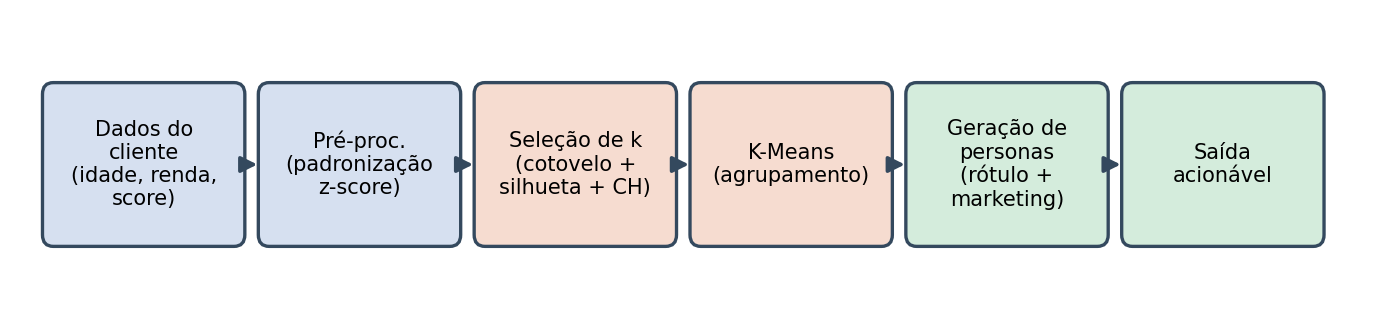
\includegraphics[width=\columnwidth]{figuras/fig_arch.png}
\caption{Arquitetura do sistema de segmenta\c{c}\~ao. Diagrama elaborado pelos autores (Matplotlib).}
\label{fig:arch}
\end{figure}

\section{Metodologia}
O sistema proposto foi concebido como um \textit{pipeline} de processamento que transforma dados brutos de clientes em personas acion\'aveis. A Fig.~\ref{fig:arch} apresenta a arquitetura, composta por seis est\'agios.

\subsection{Entrada e pr\'e-processamento}
A entrada \'e composta por tr\^es atributos por cliente: idade, renda anual e \textit{spending score} (\'indice de gasto de 1 a 100). Como esses atributos possuem escalas distintas e o K-Means se baseia em dist\^ancia euclidiana, aplica-se padroniza\c{c}\~ao \textit{z-score}, de modo que cada atributo passe a ter m\'edia zero e desvio-padr\~ao unit\'ario, evitando que a vari\'avel de maior amplitude domine o agrupamento.

\subsection{Sele\c{c}\~ao do n\'umero de grupos}
O K-Means minimiza a in\'ercia
\begin{equation}
J = \sum_{i=1}^{n} \min_{\mu_j \in C} \lVert x_i - \mu_j \rVert^2,
\end{equation}
onde $x_i$ \'e a $i$-\'esima amostra e $\mu_j$ o centroide do grupo $C_j$. Para escolher $k$, varia-se $k \in \{2,\dots,10\}$ e, para cada valor, calculam-se: a in\'ercia (cotovelo), o coeficiente de silhueta~\cite{rousseeuw1987} e o \'indice de Calinski-Harabasz~\cite{calinski1974}. A decis\~ao final pondera os tr\^es crit\'erios: quando convergem, a escolha ganha confian\c{c}a; quando divergem, a diverg\^encia \'e analisada \`a luz da interpretabilidade dos grupos.

\subsection{Agrupamento e visualiza\c{c}\~ao}
Definido $k$, executa-se o K-Means com 50 inicializa\c{c}\~oes (\textit{k-means++}) e semente fixa para reprodutibilidade. Durante a varredura de $k \in \{2,\dots,10\}$, usam-se 20 inicializa\c{c}\~oes por valor (equil\'ibrio entre custo computacional e estabilidade); o modelo final adota 50 para maximizar a qualidade do resultado escolhido. Para visualizar os grupos, projeta-se o espa\c{c}o padronizado de tr\^es dimens\~oes em duas componentes principais via PCA~\cite{jolliffe2002}.

\subsection{Gera\c{c}\~ao de personas}
Cada grupo \'e caracterizado pelas m\'edias de seus atributos (centroide em escala original). A partir desse perfil, o sistema atribui um nome descritivo e uma recomenda\c{c}\~ao de marketing, traduzindo o resultado estat\'istico em a\c{c}\~ao de neg\'ocio (p.\,ex., alta renda e alto gasto $\rightarrow$ programa \textit{premium}).

\subsection{Materiais}
O sistema foi implementado em Python com \textit{scikit-learn}~\cite{pedregosa2011}, \textit{pandas} e \textit{matplotlib}. Utilizou-se o \textit{Mall Customer Segmentation Dataset}, com 200 clientes.

\section{Experimentos}
O experimento principal consistiu em executar o \textit{pipeline} completo sobre o conjunto de dados e avaliar os tr\^es crit\'erios de sele\c{c}\~ao de $k$. A Tabela~\ref{tab:crit} consolida os valores obtidos; a Fig.~\ref{fig:crit} mostra as curvas correspondentes. Em seguida, fixou-se $k$ e analisou-se a separa\c{c}\~ao dos grupos no espa\c{c}o PCA e os perfis resultantes.

% Tabela I
\begin{table}[t]
\caption{Crit\'erios de sele\c{c}\~ao de $k$ (valores em negrito indicam o \'otimo de cada crit\'erio: cotovelo em $k=5$, silhueta e Calinski-Harabasz em $k=6$).}
\label{tab:crit}
\centering
\small
\begin{tabular}{cccc}
\toprule
$k$ & In\'ercia (WCSS) & Silhueta & Calinski-Harabasz \\
\midrule
2 & 389{,}39 & 0{,}3355 & 107{,}10 \\
3 & 295{,}21 & 0{,}3578 & 101{,}69 \\
4 & 205{,}23 & 0{,}4040 & 125{,}68 \\
5 & \textbf{168{,}25} & 0{,}4166 & 125{,}10 \\
6 & 133{,}87 & \textbf{0{,}4274} & \textbf{135{,}10} \\
7 & 117{,}01 & 0{,}4172 & 132{,}77 \\
8 & 103{,}83 & 0{,}4087 & 131{,}07 \\
9 & 92{,}35 & 0{,}4201 & 131{,}24 \\
10 & 81{,}99 & 0{,}3973 & 133{,}38 \\
\bottomrule
\end{tabular}
\end{table}

% Figura 2
\begin{figure}[t]
\centering
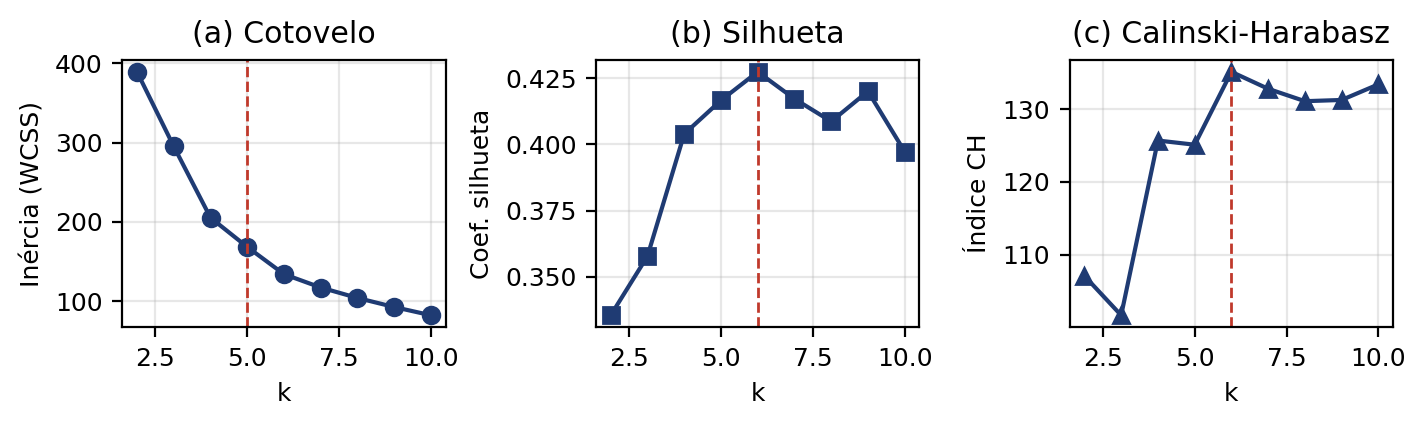
\includegraphics[width=\columnwidth]{figuras/fig_criteria.png}
\caption{Crit\'erios para sele\c{c}\~ao de $k$: (a) cotovelo, (b) silhueta e (c) Calinski-Harabasz. Linhas tracejadas marcam pontos de interesse. Figura elaborada pelos autores.}
\label{fig:crit}
\end{figure}

\section{Resultados e Discuss\~ao}
\subsection{Escolha de $k$ e diverg\^encia entre crit\'erios}
Os crit\'erios n\~ao foram un\^animes. O m\'etodo do cotovelo (Fig.~\ref{fig:crit}a) exibe inflex\~ao clara em torno de $k=5$, ponto a partir do qual a redu\c{c}\~ao da in\'ercia desacelera. J\'a a silhueta e o \'indice Calinski-Harabasz atingem m\'aximo em $k=6$ (Tabela~\ref{tab:crit}), embora a diferen\c{c}a para $k=5$ seja pequena (silhueta $0{,}4274$ contra $0{,}4166$). Trata-se justamente do cen\'ario de \textit{diverg\^encia} previsto no projeto: optou-se por $k=5$, pois o ganho marginal em $k=6$ \'e modesto e os cinco grupos resultantes possuem interpreta\c{c}\~ao de neg\'ocio mais n\'itida, ao passo que o sexto grupo tende a subdividir um perfil j\'a coeso. Essa escolha privilegia a parcim\^onia e a acionabilidade sem perda relevante de qualidade num\'erica. Em termos comparativos, o coeficiente de silhueta obtido ($0{,}42$ para $k=5$; $0{,}43$ para $k=6$) enquadra-se na faixa \textit{razo\'avel} da escala de Rousseeuw~\cite{rousseeuw1987}, que considera valores entre $0{,}41$ e $0{,}60$ indicativos de estrutura moderada a boa --- resultado alinhado com trabalhos que aplicam K-Means a dados demogr\'aficos e comportamentais de escala similar~\cite{sinaga2020,ezenkwu2015}.

% Figura 3
\begin{figure}[ht]
\centering
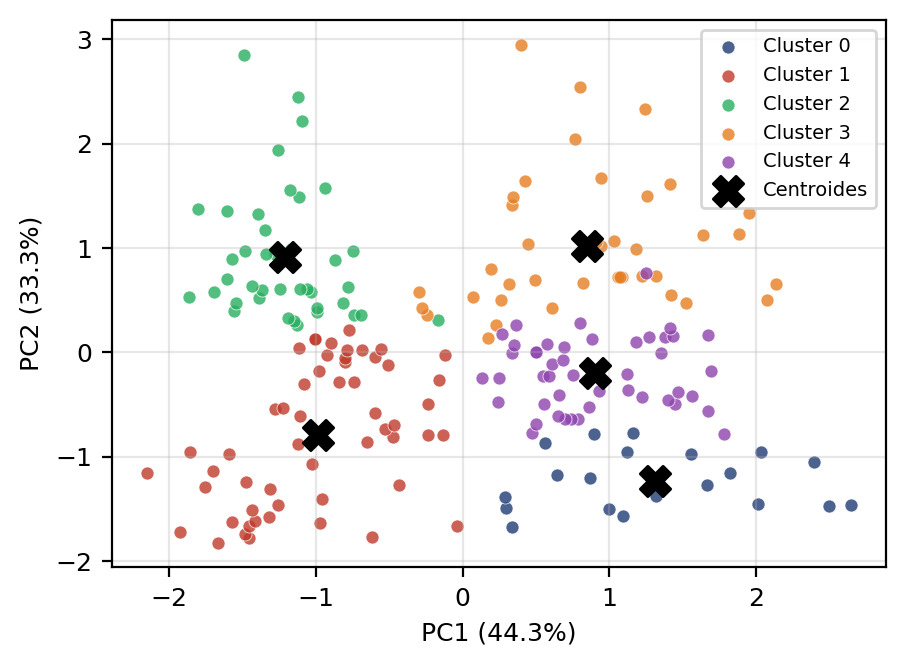
\includegraphics[width=0.82\columnwidth]{figuras/fig_pca.png}
\caption{Grupos no espa\c{c}o das duas primeiras componentes principais (PCA), com centroides destacados. Figura elaborada pelos autores.}
\label{fig:pca}
\end{figure}

\subsection{Estrutura dos grupos}
A Fig.~\ref{fig:pca} mostra os grupos projetados nas duas primeiras componentes principais, que ret\'em $77{,}6\%$ da vari\^ancia total ($44{,}3\%$ e $33{,}3\%$). Os grupos aparecem bem delimitados, com centroides distantes entre si, o que corrobora a coes\~ao indicada pela silhueta de $0{,}42$ obtida em $k=5$.

\subsection{Personas acion\'aveis}
A Tabela~\ref{tab:persona} traduz cada centroide em uma persona com recomenda\c{c}\~ao de marketing. O sistema distingue, por exemplo, clientes de alta renda com alto gasto (alvo de programas \textit{premium}) de clientes de alta renda com baixo gasto (alvo de campanhas de convers\~ao), perfis que exigem estrat\'egias opostas apesar de renda semelhante.

% Tabela II
\begin{table*}[t]
\caption{Personas geradas a partir dos centroides ($k=5$). Valores m\'edios em escala original.}
\label{tab:persona}
\centering
\small
\begin{tabular}{clccccp{5.6cm}}
\toprule
Grupo & Persona & Idade & Renda (k\$) & Gasto & $N$ & Recomenda\c{c}\~ao de marketing \\
\midrule
0 & Maduro econ\^omico & 46{,}2 & 26{,}8 & 18{,}4 & 20 & Ofertas de baixo custo e descontos sazonais; baixa prioridade de investimento. \\
1 & Jovem entusiasta & 25{,}2 & 41{,}1 & 62{,}2 & 54 & Programa de fidelidade e engajamento digital; alto potencial de longo prazo. \\
2 & \textit{Premium} ativo & 32{,}9 & 86{,}1 & 81{,}5 & 40 & Servi\c{c}os exclusivos, lan\c{c}amentos e \textit{cross-selling} de alto valor. \\
3 & Conservador endinheirado & 39{,}9 & 86{,}1 & 19{,}4 & 39 & Campanhas de convers\~ao e benef\'icios para estimular gasto; foco em confian\c{c}a. \\
4 & P\'ublico m\'edio & 55{,}6 & 54{,}4 & 48{,}9 & 47 & Comunica\c{c}\~ao equilibrada e promo\c{c}\~oes generalistas; segmento de manuten\c{c}\~ao. \\
\bottomrule
\end{tabular}
\end{table*}

\subsection{Limita\c{c}\~oes}
O sistema usa apenas tr\^es atributos e um conjunto de dados de pequeno porte (200 clientes). O K-Means assume grupos aproximadamente esf\'ericos e \'e sens\'ivel a \textit{outliers}. Trabalhos futuros podem incorporar mais atributos comportamentais, comparar com algoritmos baseados em densidade e validar as personas com dados reais de campanha.

\section{Conclus\~ao}
Apresentou-se um sistema de segmenta\c{c}\~ao de clientes estruturado como \textit{pipeline}, cujo n\'ucleo \'e o K-Means. As duas contribui\c{c}\~oes --- sele\c{c}\~ao de $k$ por tr\^es crit\'erios e gera\c{c}\~ao de personas acion\'aveis --- mostraram-se efetivas: o sistema produziu cinco perfis interpret\'aveis (silhueta $0{,}42$) e recomenda\c{c}\~oes de marketing coerentes. O caso de diverg\^encia entre crit\'erios ($k=5$ vs.\ $k=6$) evidenciou o valor da abordagem multicrit\'erio, que combina evid\^encia num\'erica e interpretabilidade na decis\~ao final.

\clearpage 

\begin{thebibliography}{00}
\bibitem{macqueen1967} J. MacQueen, ``Some methods for classification and analysis of multivariate observations,'' in \textit{Proc. 5th Berkeley Symp. Math. Statist. Probab.}, vol. 1, 1967, pp. 281--297.
\bibitem{rousseeuw1987} P. J. Rousseeuw, ``Silhouettes: A graphical aid to the interpretation and validation of cluster analysis,'' \textit{J. Comput. Appl. Math.}, vol. 20, pp. 53--65, 1987.
\bibitem{calinski1974} T. Cali\'nski and J. Harabasz, ``A dendrite method for cluster analysis,'' \textit{Commun. Statist.}, vol. 3, no. 1, pp. 1--27, 1974.
\bibitem{jolliffe2002} I. T. Jolliffe, \textit{Principal Component Analysis}, 2nd ed. New York: Springer, 2002.
\bibitem{pedregosa2011} F. Pedregosa \textit{et al.}, ``Scikit-learn: Machine learning in Python,'' \textit{J. Mach. Learn. Res.}, vol. 12, pp. 2825--2830, 2011.
\bibitem{sinaga2020} K. P. Sinaga and M.-S. Yang, ``Unsupervised K-means clustering algorithm,'' \textit{IEEE Access}, vol. 8, pp. 80436--80451, 2020.
\bibitem{ezenkwu2015} C. P. Ezenkwu, S. Ozuomba, and C. Kalu, ``Application of K-Means algorithm for efficient customer segmentation: A strategy for targeted customer services,'' \textit{Int. J. Adv. Res. Artif. Intell.}, vol. 4, no. 10, pp. 40--44, 2015.
\end{thebibliography}

\newpage

\section*{Anexo --- Declara\c{c}\~ao de Uso de Intelig\^encia Artificial}
\textbf{Ferramenta utilizada:} assistente de IA baseado em modelo de linguagem (Claude, Anthropic).

\textbf{Finalidade do uso:} revis\~ao gramatical e ortogr\'afica do texto redigido pelos autores, organiza\c{c}\~ao de ideias e aux\'ilio no c\'odigo Python do \textit{pipeline} experimental.

\textbf{Forma de utiliza\c{c}\~ao:} o texto do artigo foi elaborado pelos integrantes do grupo; a ferramenta foi utilizada para revis\~ao e sugest\~oes de melhoria de escrita, sem gera\c{c}\~ao autom\'atica de conte\'udo. No c\'odigo, a IA auxiliou na organiza\c{c}\~ao do \textit{pipeline}, que foi executado e verificado pelos autores. Todos os resultados num\'ericos (Tabelas~\ref{tab:crit} e \ref{tab:persona}) e as figuras foram produzidos pela execu\c{c}\~ao do c\'odigo sobre o conjunto de dados real e conferidos pelo grupo. Os diagramas e gr\'aficos (Figs.~\ref{fig:arch}--\ref{fig:pca}) foram gerados programaticamente com a biblioteca Matplotlib, possuindo legenda e numera\c{c}\~ao; o conte\'udo conceitual associado est\'a referenciado na bibliografia. A decis\~ao metodol\'ogica final e a interpreta\c{c}\~ao dos resultados s\~ao de responsabilidade dos autores.

\end{document}
